\documentclass[10pt,a4paper]{article}
\usepackage[utf8]{inputenc}
\usepackage[catalan]{babel}
\usepackage{multicol}
\usepackage{graphicx}
\usepackage{fancyhdr}
\usepackage{times}
\usepackage{titlesec}
\usepackage{multirow}
\usepackage{lettrine}
\usepackage[top=2cm, bottom=1.5cm, left=2cm, right=2cm]{geometry}
\usepackage[figurename=Fig.,tablename=TAULA]{caption}
\usepackage{hyperref}
\usepackage[ampersand]{easylist}

\titlespacing*{\section}{0pt}{0.5cm}{0.2cm}
\titlespacing*{\subsection}{0pt}{0.5cm}{0.2cm}


\graphicspath{{img/}}

\author{\normalsize\sffamily Kevin Martín Fernández}
\title{\huge{\sffamily Informe inicial: Entorn de simulació per la captura d'imatges des de dron}}
\date{}

\newcommand\blfootnote[1]{%
  \begingroup
  \renewcommand\thefootnote{}\footnote{#1}%
  \addtocounter{footnote}{-1}%
  \endgroup
}

%
%\large\bfseries\sffamily
\titleformat{\section}
{\large\sffamily\scshape\bfseries}
{\textbf{\thesection}}{1em}{}

\begin{document}

\fancyhead[LO]{\scriptsize Kevin Martín: Informe inicial: Entorn de simulació per la captura d'imatges des de dron}
\fancyhead[RO]{\thepage}
\fancyhead[L]{\thepage}
\fancyhead[R]{\scriptsize EE/UAB TFG INFORMÀTICA: Entorn de simulació per la captura d'imatges des de dron}

\fancyfoot[CO,C]{}

\fancypagestyle{primerapagina}
{
   \fancyhf{}
   \fancyhead[L]{\scriptsize TFG EN ENGINYERIA INFORMÀTICA, ESCOLA D'ENGINYERIA (EE), UNIVERSITAT AUTÒNOMA DE BARCELONA (UAB)}
   \fancyfoot[C]{\scriptsize ``Mes'' de 2019, Escola d'Enginyeria (UAB)}
}

%\lhead{\thepage}
%\chead{}
%\rhead{\tiny EE/UAB TFG INFORMÀTICA: TÍTOL (ABREUJAT SI ÉS MOLT LLARG)}
%\lhead{ EE/UAB \thepage}
%\lfoot{}
%\cfoot{\tiny{February 2015, Escola d'Enginyeria (UAB)}}
%\rfoot{}
\renewcommand{\headrulewidth}{0pt}
\renewcommand{\footrulewidth}{0pt}
\pagestyle{fancy}

%\thispagestyle{myheadings}
{
\maketitle
}

\thispagestyle{primerapagina}
%\twocolumn[\begin{@twocolumnfalse}
%\maketitle
%\begin{abstract}
\begin{center}
\parbox{0.915\textwidth}

\end{center}

\bigskip
%\end{abstract}

\vspace{-1cm}
\section{Introducció}

\lettrine[lines=2]{L}{a} simulació de espais per a la generació de imatges artificials és un àmbit en el que es busca representa el mon real de la forma més realista possible per tal de poder generar informació que en entorns reals ens representaria un perill o un cost econòmic elevat.
\\
\\
En aquest treball és vol aconseguir que mitjançant dades de mapes d'elevacions i imatges aèries de terrenys reals generar-ho en un entorn simulat per tal de poder generar imatges fictícies amb la màxima realitat possible per tal de generar datasets d'imatges per la utilització en diversos camps del aprenentatge computacional.

\section{Objectius}

En aquest apartat determinarem els diferents objectius del projecte en format de jerarquia per tal de veure la dependència entre els diferents objectius:

\begin{easylist}
\ListProperties(Progressive*=0.5cm)
& Analitzar
&& Investigar l'estat de l'art
&&& Estudiar AirSim
&&& Estudiar Carla SIMULATOR
&&& Estudiar proposta pròpia
&& Definir els objectius
&& Investigar motors gràfics
&&& Investigar Unreal Engine
&&& Investigar altres motors gràfics
&& Investigar els mapes d'altura
&& Investigar les imatges tant RGB com multi-espectrals
&& Investigar webservices WMS
&& Investigar llibreries RCP
& Definir
&& Definir mòduls interessants pel projecte
&& Definir l'estructura del software
&& Definir plataformes utilitzades
&&& Definir els mòduls a desenvolupar
&&& Definir la comunicació entre els mòduls
&&& Definir estructura de les dades que rebrà Unreal Engine
& Desenvolupar
&& Desenvolupar modul de transformació i obtenció de dades
&&& Desenvolupar el modul de transformació de dades d'altura i textures
&&& Desenvolupar l'importador de dades en Unreal Engine
&& Desenvolupar modul gràfic (Ureal Engine)
&&& Desenvolupar la interfície del menú
&&& Desenvolupar el mòdul per importar fitxers personalitzats en Unreal Engine
&&& Desenvolupar codi per la generació del terreny
&&& Desenvolupar codi per la generació dels materials
&&&& Visualitzar diferents materials (RGB, Multiespectre, etc)
&&& Desenvolupar codi  de servidor per control del vehicle
&& Desenvolupar modul de scripting
&&& Desenvolupament client que controlara el vehicle
&& Integrar els mòduls de AirSim en Unreal Engine
&&& Integrar modul de Drons en el projecte
&&& Integrar modul de Segmentació en el projecte
&& Desenvolupar altres capes d'informació
& Testejar
&& Fer provàs del modul de transformació de dades
&&& Provar amb dades locals
&&& Provar amb dades externes
&& Fer provàs del modul gràfic 
&& Fer provàs del modul de control per scripting
&&& Elaborar script d'exemple
&&& Provar script d'exemple
& Documentar
&& Redactar informe inicial
&& Redactar informe de seguiment I
&& Redactar informe de seguiment II
&& Redactar el informe final
&& Elaborar proposta de presentació
&& Elaborar pòster
&& Gestionar la documentació del dossier
\end{easylist}

\section{Estat de l'art}
\label{estatart}

Actualment existeixen diverses aplicacions per la generació d'imatges en entorns que simulen la realitat amb la finalitat de generar dades per algoritmes d'aprenentatge.
En aquest àmbit unes de les més importants és AirSim \cite{airsim} desenvolupat per Microsoft sobre el motor gràfic Unreal Engine aquest entorn permet la simulació de cotxes i drons, control per scripts, simulació climatològica, simulació del sol, generació d'imatges en visualització com son rgb, segmentació o profunditat, etc... Per altra banda un altre entorn similar al anterior és Carla SIMULATOR \cite{carla} aquest software esta enfocat en cotxes ja que el seu principal objectiu es obtenir dades per l'aprenentatge de cotxes autònoms.

\subsection{AirSim}
AirSim es un simulador gràfic elaborat en Unreal Engine \cite{unreal} aquest simulador té la finalitat de generar imatges en un entorn totalment fictici, incorpora diversos mòduls que ens ofereix les següents funcionalitats (podem veure un exemple a la figura \ref{fig-airsim}):
\\
\begin{easylist}[itemize]
& Simulació de cotxes
& Simulació de drons
& Compatibilitat amb controladors reals de drons
& Gravació 
& Vista de mapa de profunditats
& Vista segmentada
& Efectes de pluja
& Control d'il·luminació segons l'hora diària
& Control dels vehicles mitjançant scripts en python
\end{easylist}

\begin{figure}[!h]
\centering
  	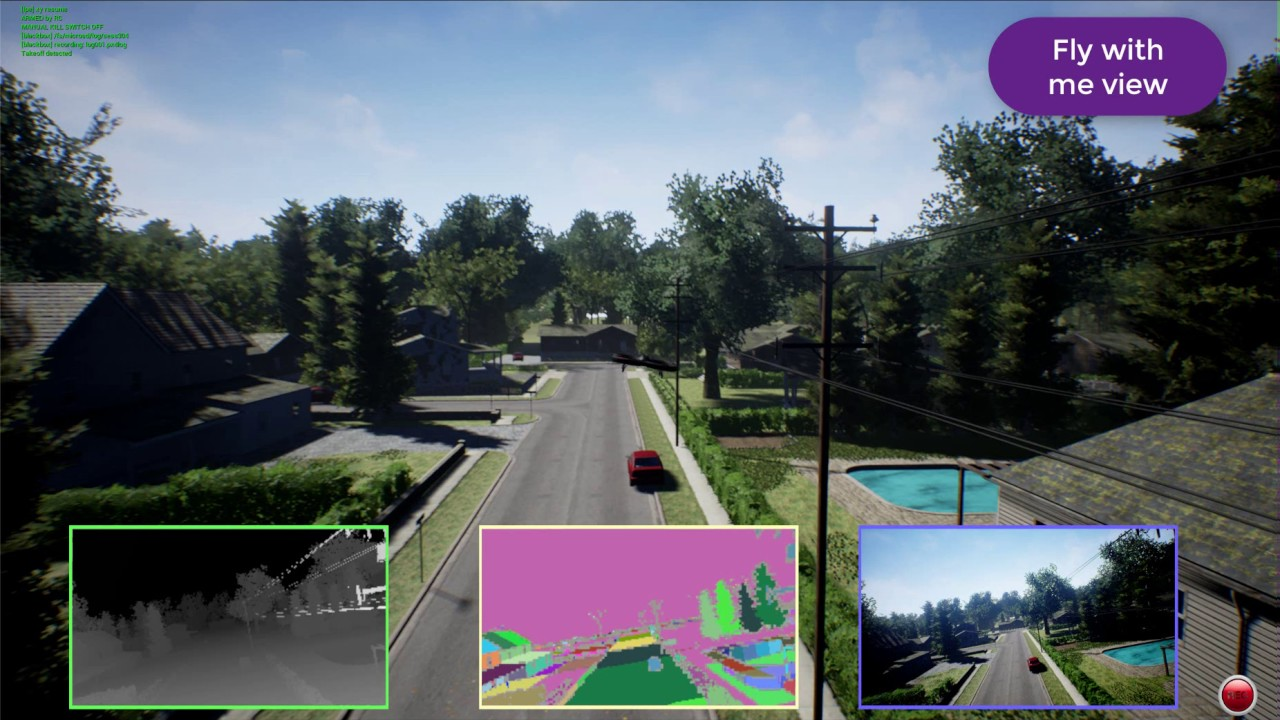
\includegraphics[width=0.4\textwidth]{airsim}
	\caption{Simulador Airsim}
	\label{fig-airsim}
\end{figure}

\newpage
\subsection{Carla SIMULATOR}
Carla es un simulador gràfic elaborat en Unreal Engine \cite{unreal} aquesta simulador té la finalitat de generar imatges en entorn fictici amb la màxima realitat possible per generar imatges que serveixin per l'aprenentatge de xarxes neuronals capaces de conduir un cotxe autònom de forma segura tenint en compte els casos poc probables que no es podrien generar en un entorn físic. Aquest entorn compte amb les següents funcionalitats:

\begin{easylist}[itemize]
& Simulació de cotxes
& Vista de mapa de profunditats
& Vista segmentada
& Simulació de trafic
& Control dels actors amb scripts de python
\end{easylist}

\section{Estructura d'altres projectes}

Per tal de determinar la estructura del nostre projecte s'han estudiat varies alternatives vistes al apartat \ref{estatart} en les quals es pot veure com estan organitzats altres projectes similars. En aquest apartat veurem l'estructura de diferents projectes amb l'objectiu de decidir l'estructura del projecte y diferents llibreries.

\subsection{AirSim} 

AirSim esta composat per múltiples mòduls escrits en diversos llenguatges com es pot veure a continuació:\\

\begin{easylist}[itemize]
& AirLib (C++): Modul per a Unreal Engine que proporciona les classes bàsiques per comunicar-se mitjançant el protocol RCP i control dels vehicles simulats.
& DroneServer (C++): Servidor per rebre ordres de Dron mitjançant RCP
& DroneShell (C++): Client de consola per enviar ordres al modul de dron.
& PythonClient (Python): Client que envia ordres mitjançant RCP, també incorpora codi per el tractament, segmentació d'imatges, etc.
& SGM (C++): Codi per tractar imatges i generar les les vistes segmentada i stereo. 
& Unity (C\# i C++): Demostració en el motor gràfic Unity, incorpora una serie de mòduls per Unity per visualitzar la informació de AirSim.
& Unreal Engine (C++): Demostració en el motor gràfic Unreal Engine, incorpora una serie de mòduls per Unreal Engine per visualitzar la informació de AirSim.
\end{easylist}

\subsection{Carla SIMULATOR}

Carla SIMULATOR esta composat per múltiples mòduls com podem veure en la figura \ref{fig-carlamodules} escrits en diversos llenguatges com es pot veure a continuació:

\begin{figure}[!h]
\centering
  	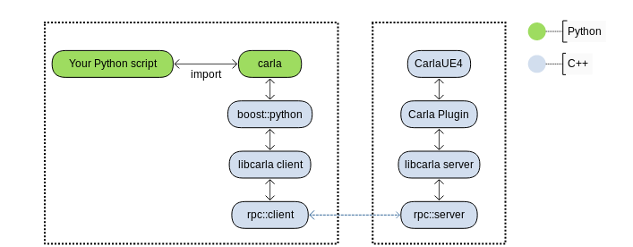
\includegraphics[width=0.6\textwidth]{carlamodules}
	\caption{Relació entre els mòduls de Carla}
	\label{fig-carlamodules}
\end{figure}

\begin{easylist}[itemize]
& LibCarla (C++): Llibreria principal de Carla
& Unreal (C++): Motor gràfic amb el plugin de carla, que incorpora totes les funcionalitats afegides a Unreal.
& PythonAPI (Python): API que ens permetrà enviar comandes al module de Carla que fa de servidor, aquesta api serveix per crear scripts propis.
\end{easylist}

\section{Metodologia}

En aquest projecte hem decidit utilitzar una metodologies de tipus Agile \cite{agile} ja que això ens permetrà identificar de una forma millor les petites parts de les que es composa aquest projecte, a més a més d'adaptar-se als canvis imprevistos. En concret s'ha escollit la tècnica Kanban \cite{kanban} que consisteix en organitza el nostre backlog (tasques de curta duració) en 
targetes que ficarem en un taulell segons en quin punt del cicle de vida de la tasca es trobi (pendent, començada, etc) per això s'ha decidit utilitzar l'eina Trello \cite{trello} que permet de forma visual crear targetes i moure-les entre les diferents llistes.

\subsection{Diagrama de Gant}

Per tal de gestionar el projecte també s'ha empleat un diagrama de Gant elaborat amb excel com podem veure a la figura \ref{fig-gant}. En aquest diagrama contemplarem les diverses tasques i subtasques per tal de fer una previsió del treball a realitzar, el temps aproximat que trigarem per cada tasca, això ens permetrà fer una aproximació del temps que ens comportara el projecte d'aquesta forma podrem determinar la viabilitat.

\begin{figure}[!h]
\centering
  	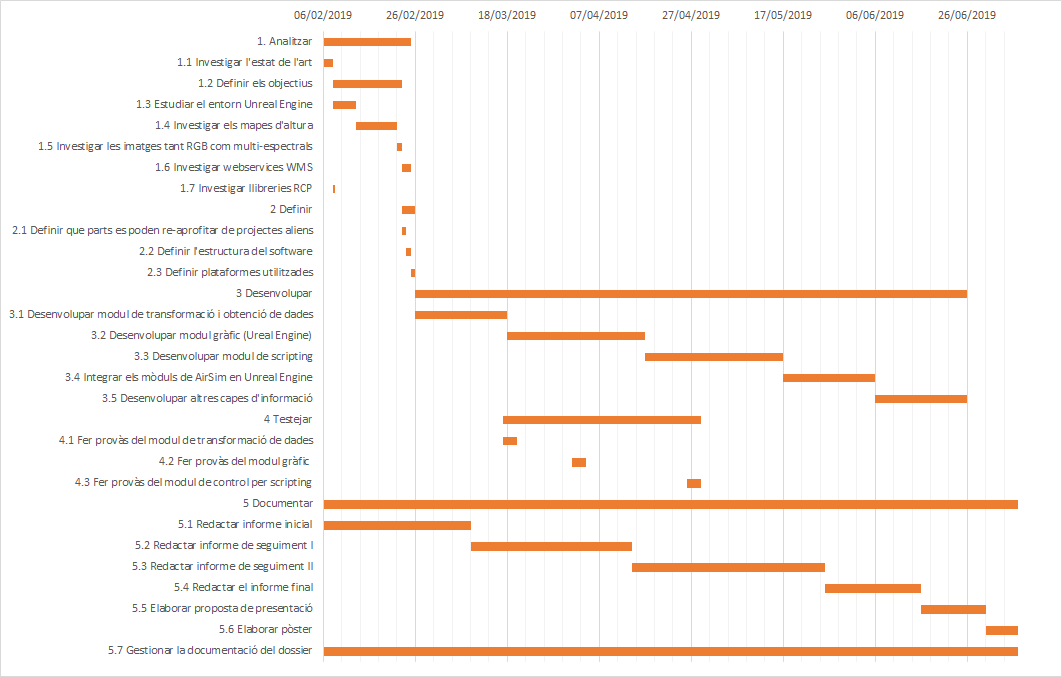
\includegraphics[width=1\textwidth]{gant}
	\caption{Diagrama de Gant}
	\label{fig-gant}
\end{figure}

\newpage
\section{Estructura escollida}

Analitzant varis projectes de característiques similar s'ha decidit per una estructura pròpia com podrem veure en la figura \ref{fig-dronsimulatormodules} podent reutilitzar alguns dels petits mòduls open-source de altres projectes. S'ha pres aquesta decisió degut a que els altres projectes es basen en crear terrenys predefinits mitjançant l'entorn de Unreal, contrari a la finalitat d'aquest projecte en el qual es volen elaborar de forma automàtica terrenys a partir de dades reals.

\begin{figure}[!h]
\centering
  	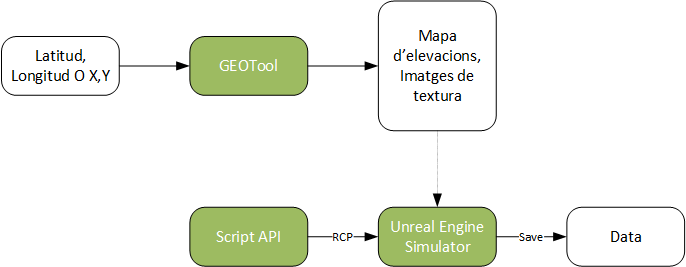
\includegraphics[width=0.8\textwidth]{structuretfg}
	\caption{Estructura DronSimulator}
	\label{fig-dronsimulatormodules}
\end{figure}

En el nostre projecte constara d'aquests mòduls:

\begin{easylist}[itemize]
& GEOTool (Python): En aquest modul es centrara en donar les eines necessàries per la obtenció y adaptació  de les dades amb l'objectiu de poder importar-les en el entorn de Unreal Engine, també pot incorporara mòduls de processament de imatge per tal d'afegir informació addicional a les textures o fer tractaments de millora d'imatges a partir de xarxes neurals.
& ScriptAPI (Python): API que ens permetrà fer scripts en Python per tal de controlar la càmera en el entorn gràfic. D'aquesta forma també ens permetrà l'obtenció d'imatges en l'entorn Unreal Engine.
& Unreal Engine Simulator (C++): Incorporara tot el motor gràfic i plugins necessaris per la comunicació amb els fitxers generats amb el mòdul GEOTool, visualització de dades, etc.
\end{easylist}


\begin{thebibliography}{11}
\bibitem{airsim}
AirSim - \url{https://github.com/Microsoft/AirSim} [19/02/2019]

\bibitem{carla}
Carla SIMULATOR - \url{http://carla.org} [19/02/2019]

\bibitem{agile}
Agile software development
\\ \url{https://en.wikipedia.org/wiki/Agile_software_development}
[19/02/2019]

\bibitem{kanban}
Kanban
\\ \url{https://www.iebschool.com/blog/metodologia-kanban-agile-scrum/} [19/02/2019]

\bibitem{trello}
Trello - \url{https://trello.com/} [19/02/2019]

\bibitem{unreal}
Unreal Engine - \url{https://www.unrealengine.com/en-US/what-is-unreal-engine-4} [09/03/2019]

\end{thebibliography}

\end{document}

